\section{Motivation}\label{motivation}

\begin{frame}[fragile]{Old Workflow - R to \LaTeX}

\begin{enumerate}
\def\labelenumi{\arabic{enumi}.}
\itemsep1pt\parskip0pt\parsep0pt
\item
  Do some cool stuff in R:
\end{enumerate}

\begin{Shaded}
\begin{Highlighting}[]
\NormalTok{mod1 <-}\StringTok{ }\KeywordTok{lm}\NormalTok{(mpg~hp, }\DataTypeTok{data =} \NormalTok{mtcars)}
\KeywordTok{with}\NormalTok{(mtcars, }\KeywordTok{plot}\NormalTok{(mpg~hp))}
\KeywordTok{abline}\NormalTok{(mod1)}
\KeywordTok{summary}\NormalTok{(mod1)}
\end{Highlighting}
\end{Shaded}

\begin{enumerate}
\def\labelenumi{\arabic{enumi}.}
\setcounter{enumi}{1}
\item
  Copy/save the output/figure.
\item
  Paste into Latex document:
\end{enumerate}

\begin{Shaded}
\begin{Highlighting}[]
\NormalTok{\textbackslash{}begin\{verbatim\}}
\NormalTok{mod1 <-}\StringTok{ }\KeywordTok{lm}\NormalTok{(mpg~hp, }\DataTypeTok{data =} \NormalTok{mtcars)}
\NormalTok{...}
\NormalTok{\textbackslash{}includegraphics\{figures/mpg.pdf\}}
\end{Highlighting}
\end{Shaded}

\end{frame}

\begin{frame}{Old Workflow - Problems}

\begin{itemize}
\item
  What if we need to make a change?
\item
  Latex is hard and requires a lot of boilerplate.
\item
  Distracting: doesn't facilitate higher-order thinking.
\end{itemize}

\end{frame}

\begin{frame}{Reproducibility}

\begin{itemize}
\item
  If I win the lottery and drop out of graduate school, could someone
  else pick up where I left off?
\item
  How long would it take them to do so?
\end{itemize}

\end{frame}

\begin{frame}{Interactivity}

\begin{itemize}
\item
  We live in the future. Why should our documents be static?
\item
  Interactive documents are useful to everyone: ourselves, our students,
  executives, etc.
\end{itemize}

\end{frame}

\section{New Workflow}\label{new-workflow}

\begin{frame}{New Workflow - Unified Document}

\begin{enumerate}
\def\labelenumi{\arabic{enumi}.}
\item
  Do some cool stuff in RMarkdown.
\item
  Push button.
\item
  Get PDF.
\end{enumerate}

\end{frame}

\begin{frame}{New Workflow - Write Code}

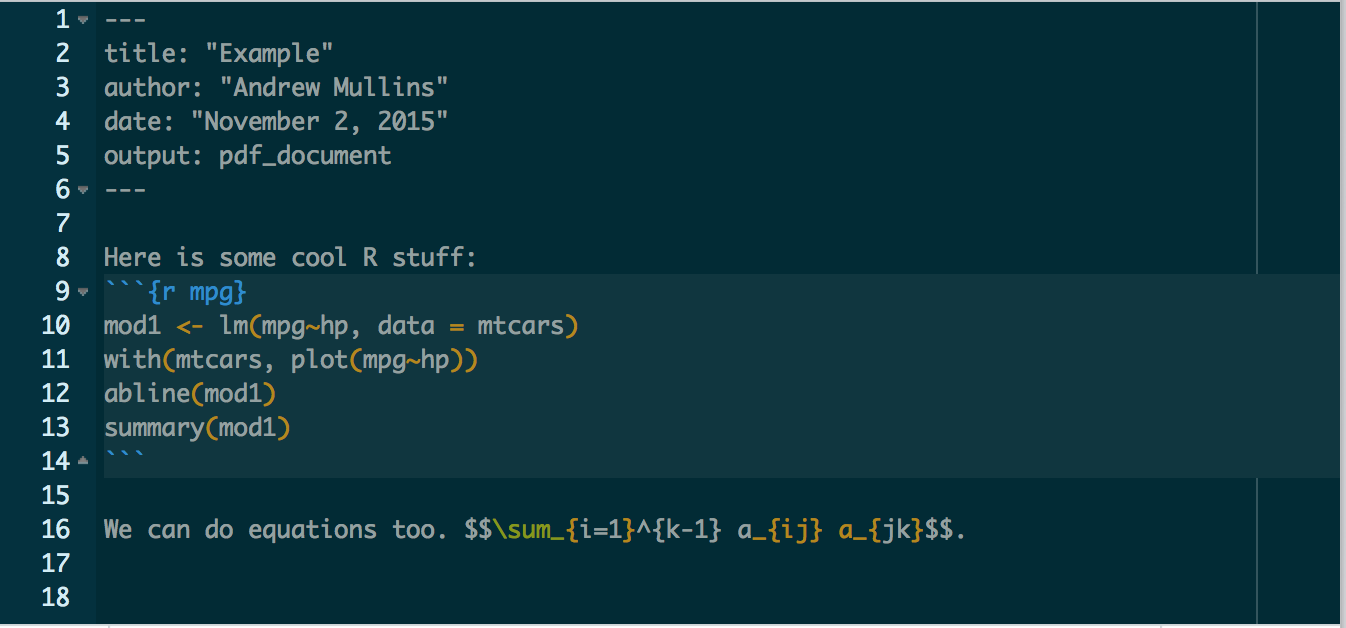
\includegraphics{images/code.png}

\end{frame}

\begin{frame}{New Workflow - Push Button}

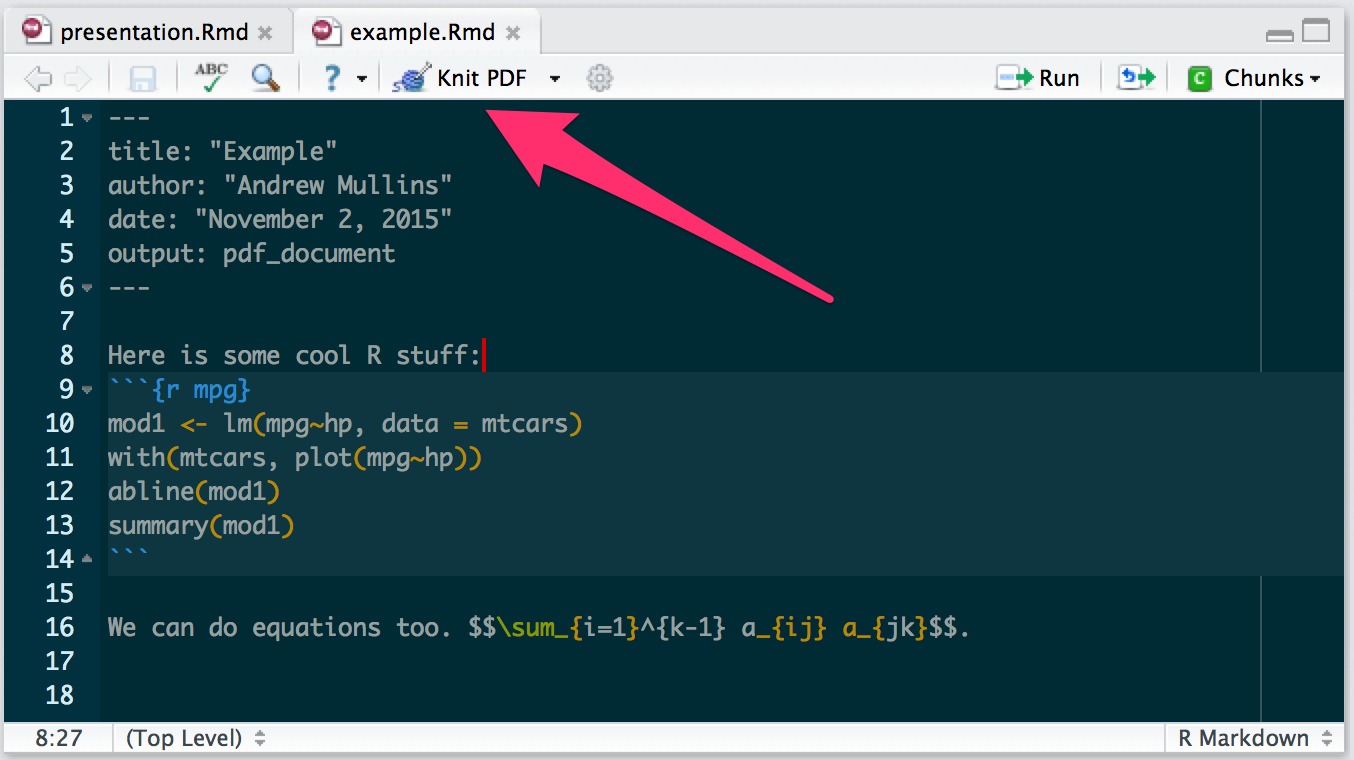
\includegraphics{images/knit.png}

\end{frame}

\begin{frame}{New Workflow - Get PDF 1}

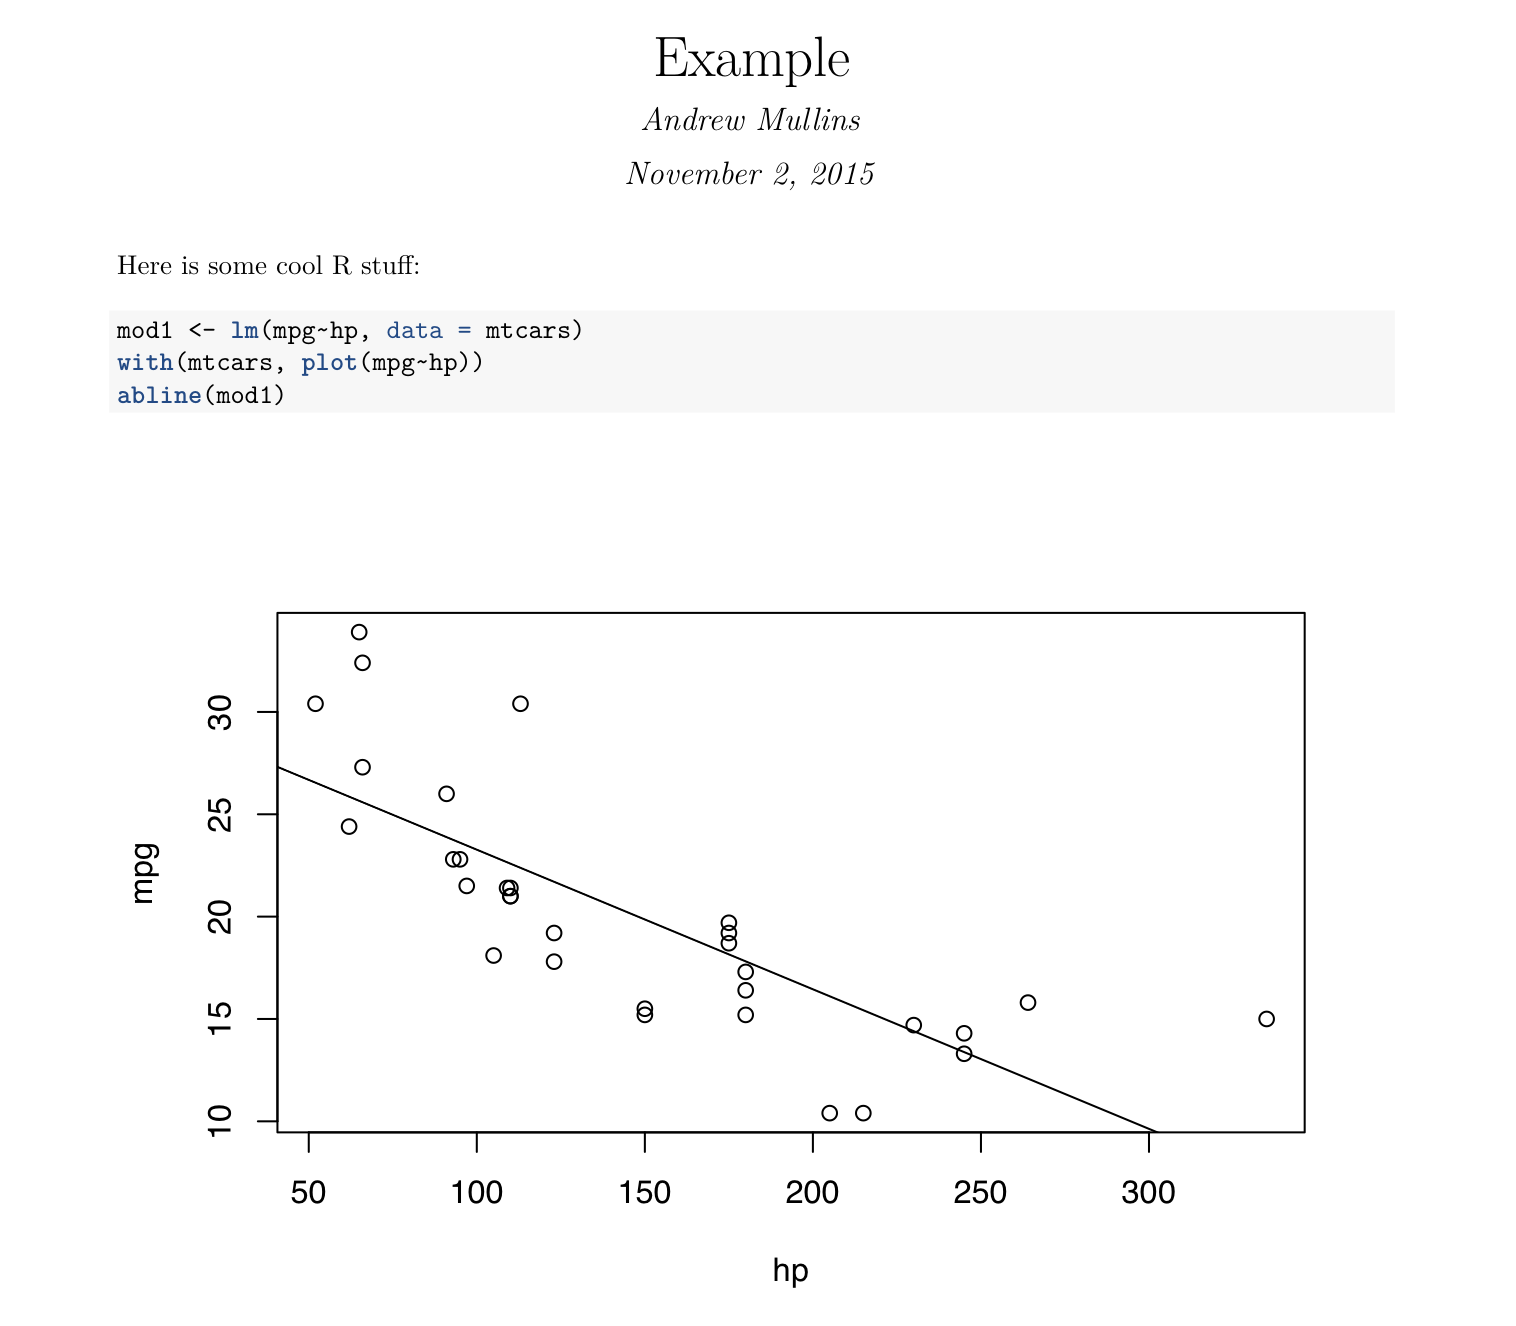
\includegraphics{images/pdf1.png}

\end{frame}

\begin{frame}{New Workflow - Get PDF 2}

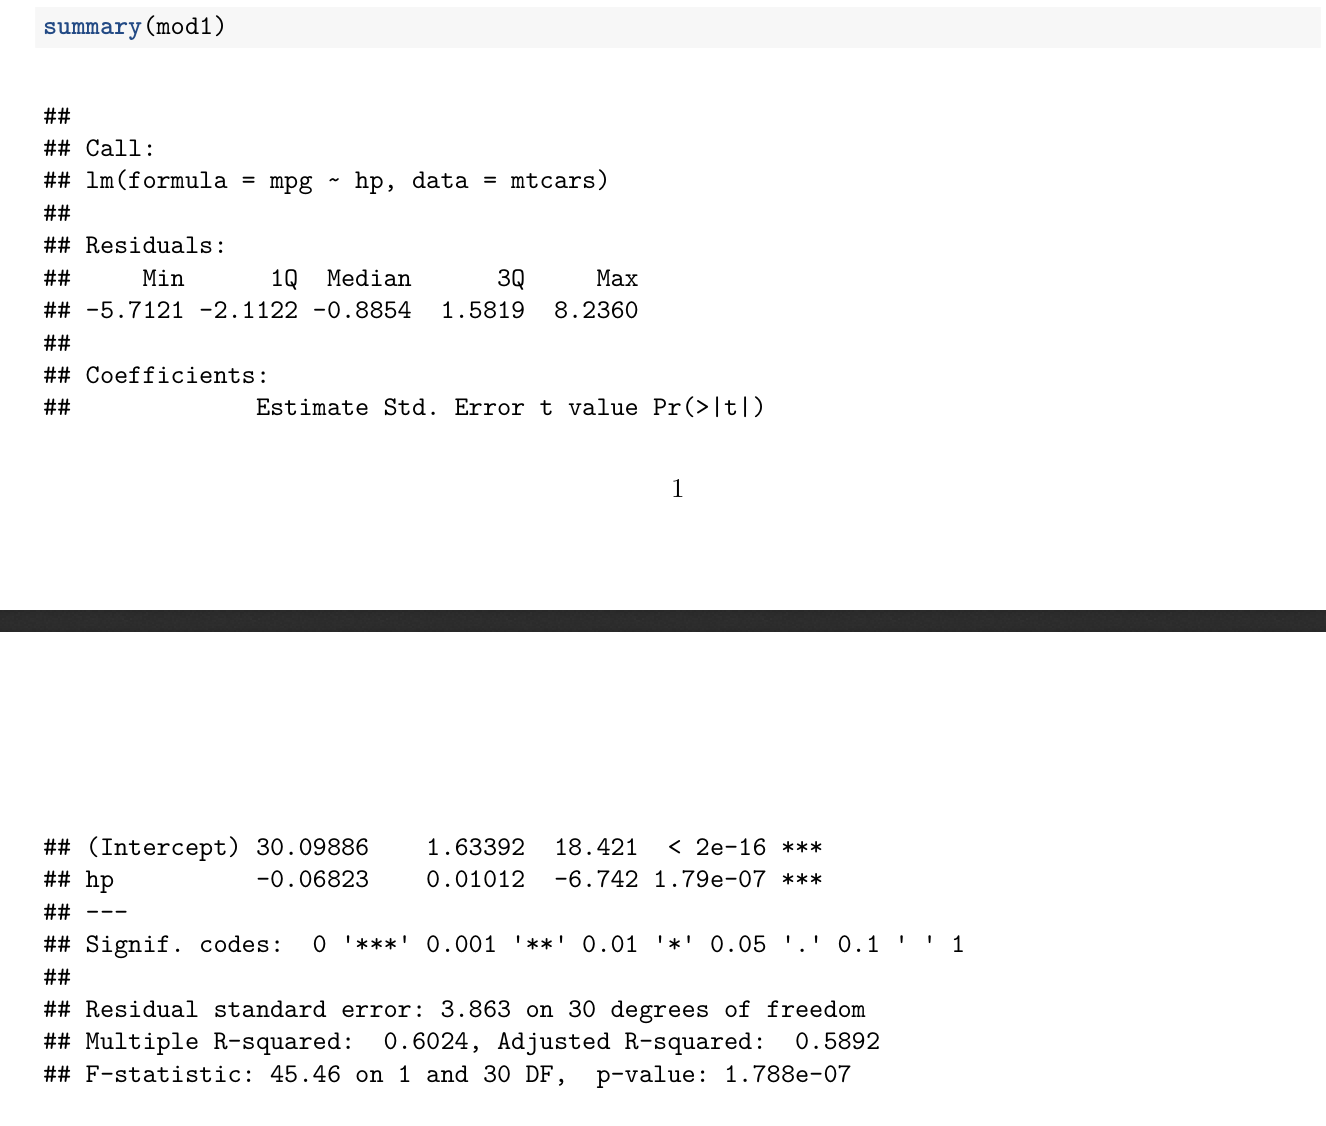
\includegraphics{images/pdf2.png}

\end{frame}

\begin{frame}{New Workflow - Get PDF 3}

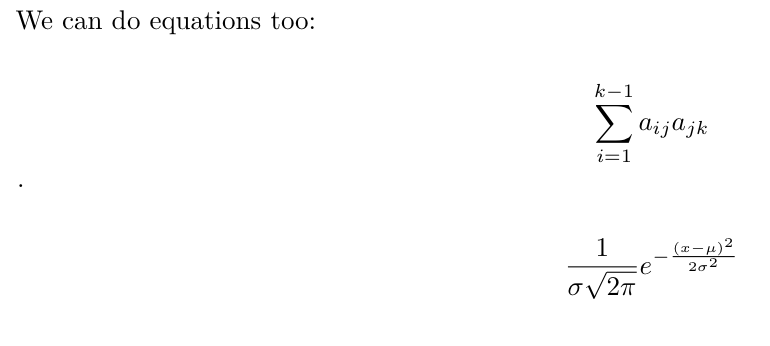
\includegraphics{images/pdf3.png}

\end{frame}

\begin{frame}{New Workflow - Make a change}

\huge{Just change it in one place and press button.}

\end{frame}

\section{Other Tools}\label{other-tools}

\begin{frame}{Sweave}

Problem: Sometimes we need the fine-tuned control you can get with
Latex.

Solution: Sweave let's use get both the power of Latex while still being
able to use in-line R code.

\end{frame}

\begin{frame}{Sweave Example Code}

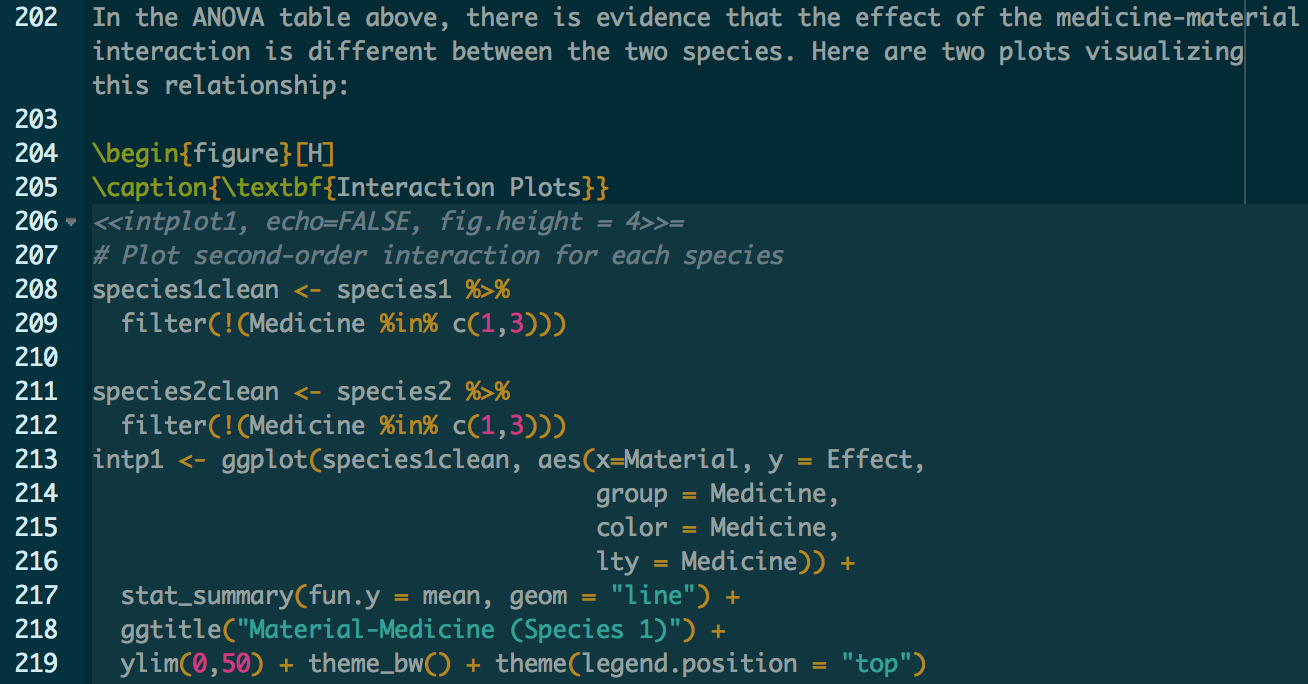
\includegraphics{images/sweave1.png}

\end{frame}

\begin{frame}{Sweave Example Output}

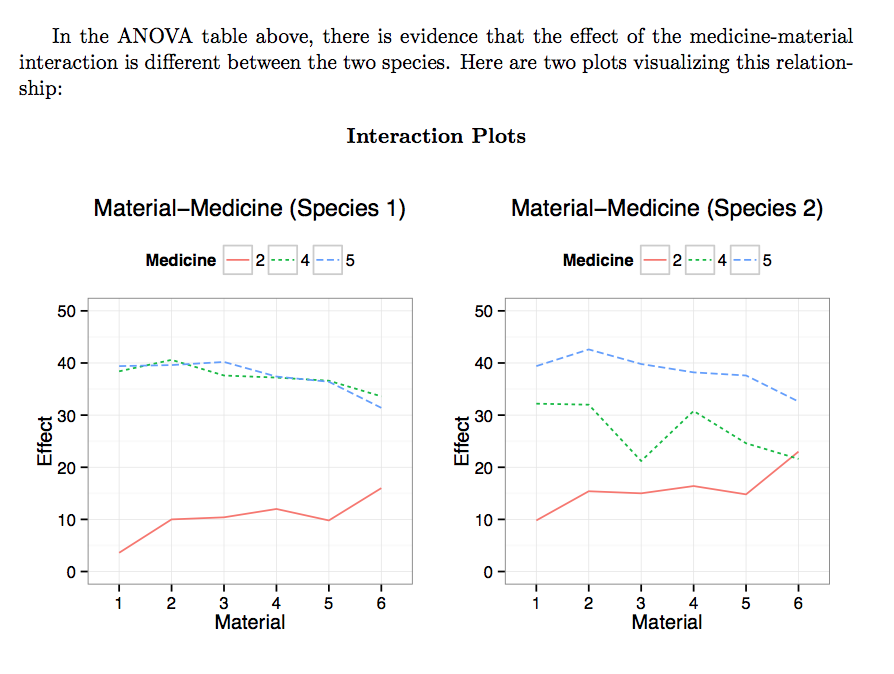
\includegraphics{images/sweave2.png}

\end{frame}

\begin{frame}{xtable/stargazer}

Problem: R output is ugly.

Solution: \texttt{xtable}/\texttt{stargazer} creates Markdown/Latex code
that is inserted into your document as-is.

\end{frame}

\begin{frame}{xtable Example Code}

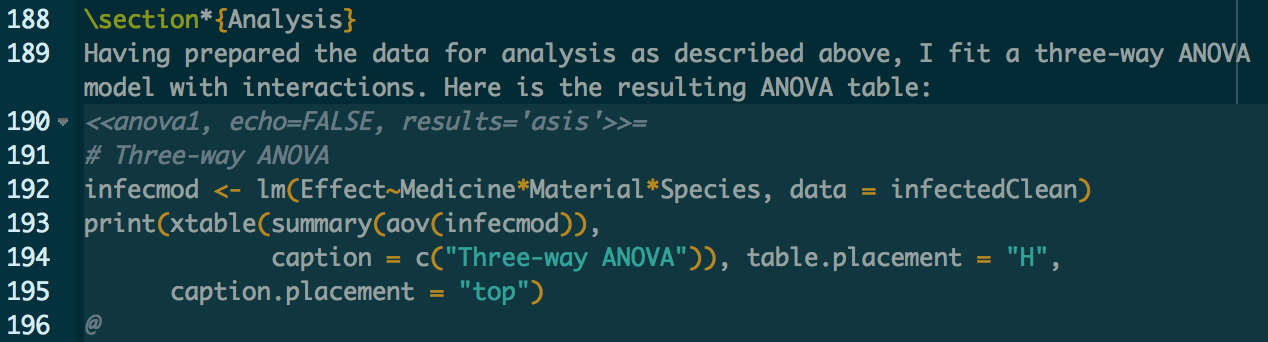
\includegraphics{images/xtable1.png}

\end{frame}

\begin{frame}{xtable Example Output}

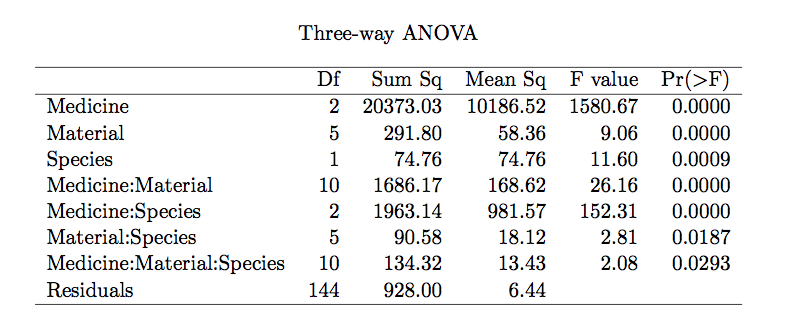
\includegraphics{images/xtable2.png}

\end{frame}

\begin{frame}{stargazer Example Code}

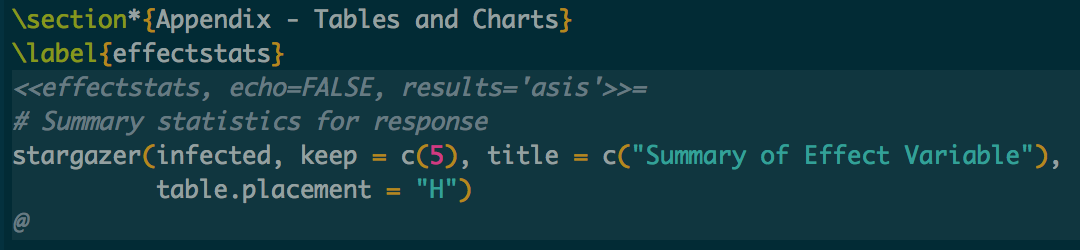
\includegraphics{images/stargazer1.png}

\end{frame}

\begin{frame}{stargazer Example Output}

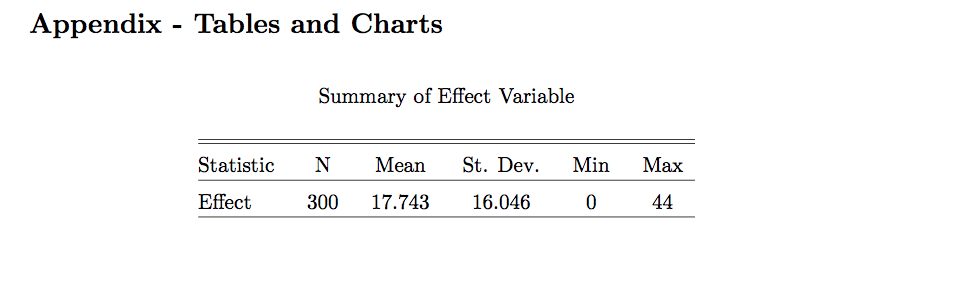
\includegraphics{images/stargazer2.png}

\end{frame}

\begin{frame}{broom}

Problem: A lot of common R objects have bizarre inner structure.

\end{frame}

\begin{frame}{broom - Example: \texttt{lm}}

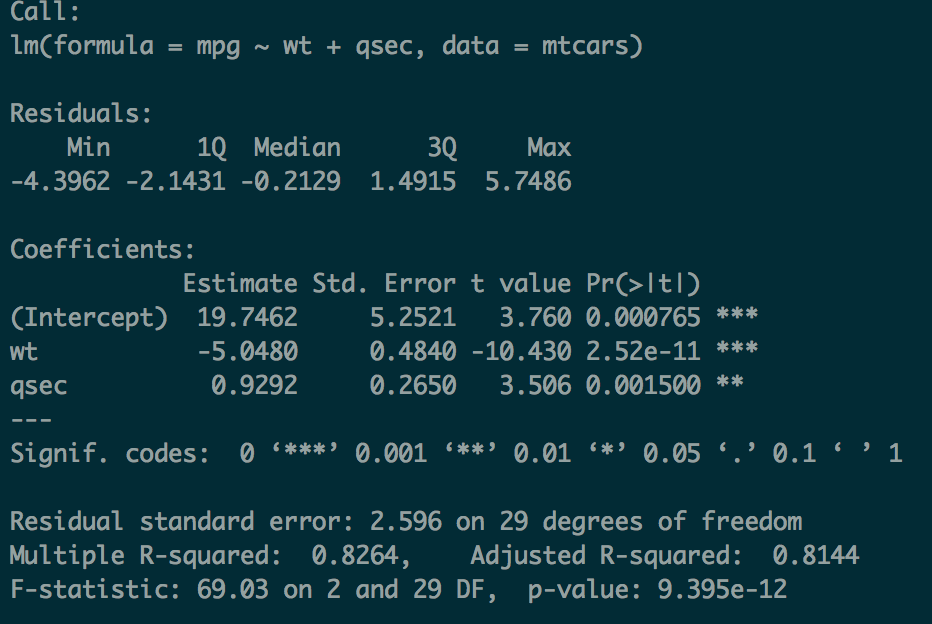
\includegraphics{images/broom1.png}

\end{frame}

\begin{frame}{broom - Example: \texttt{lm}}

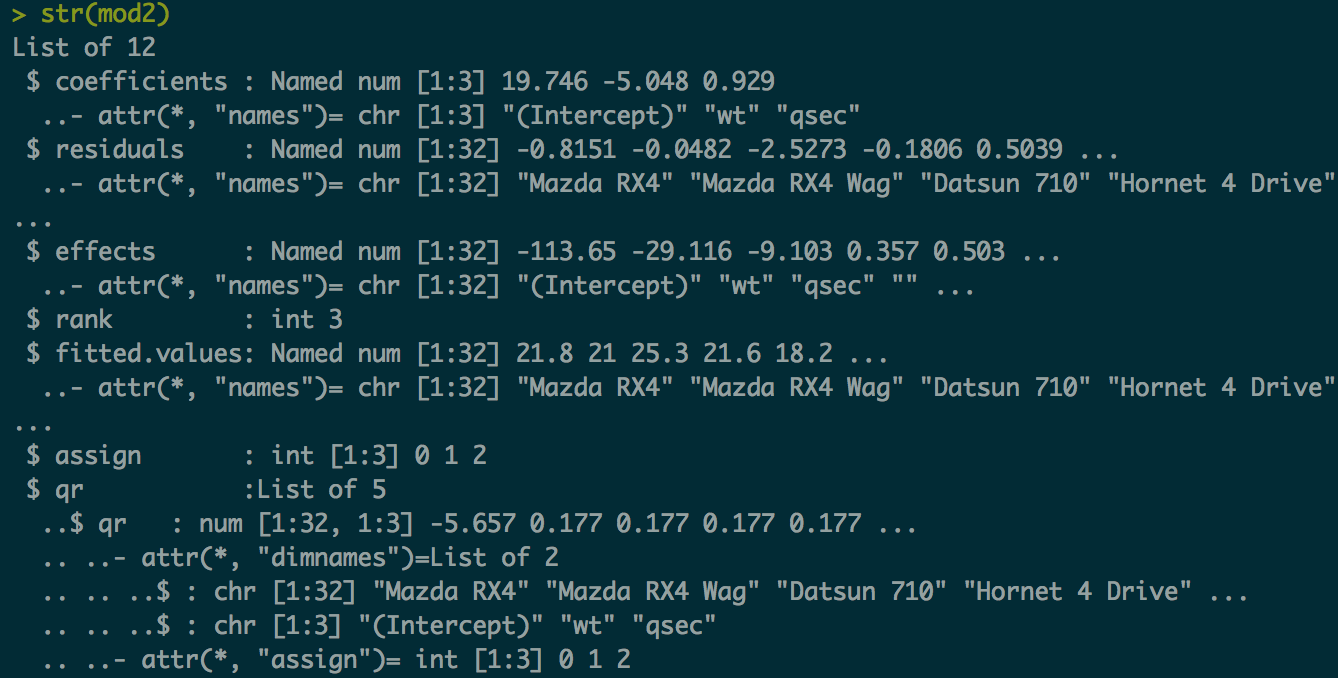
\includegraphics{images/broom2.png}

\end{frame}

\begin{frame}[fragile]{broom - Example: \texttt{lm}}

\begin{Shaded}
\begin{Highlighting}[]
\KeywordTok{library}\NormalTok{(broom)}
\KeywordTok{tidy}\NormalTok{(mod2)[,}\DecValTok{1}\NormalTok{:}\DecValTok{4}\NormalTok{]}
\end{Highlighting}
\end{Shaded}

\begin{verbatim}
##          term  estimate std.error  statistic
## 1 (Intercept) 19.746223 5.2520617   3.759709
## 2          wt -5.047982 0.4839974 -10.429771
## 3        qsec  0.929198 0.2650173   3.506179
\end{verbatim}

\end{frame}

\begin{frame}{broom - Supports}

\begin{itemize}
\itemsep1pt\parskip0pt\parsep0pt
\item
  \texttt{lm}, \texttt{glm}, \texttt{htest}, \texttt{anova},
  \texttt{nls}, \texttt{kmeans}, \texttt{manova}
\item
  \texttt{TukeyHSD}, \texttt{arima}, \texttt{lme4}, \texttt{glmnet},
  \texttt{boot}, \texttt{gam}
\item
  \texttt{survival}, \texttt{lfe}, \texttt{zoo}, \texttt{multcomp},
  \texttt{sp}, \texttt{maps}, \ldots
\end{itemize}

\end{frame}

\section{Learning More}\label{learning-more}

\begin{frame}{Examples}

\begin{itemize}
\itemsep1pt\parskip0pt\parsep0pt
\item
  These slides were created in RMarkdown
\item
  Sweave file used for Spring 2015 QEM Submission
\item
  \url{https://github.com/andrewjlm/jrcolloquium}
\end{itemize}

\end{frame}
